\subsection{Capability esterne}
Le capability esterne, come l'istituto di credito, la ditta di
spedizioni e il fornitore, sono state implementate utilizzando dei
servizi Jolie. Tali servizi sono stati semplificati: la loro
implementazione \`e difatto un semplice scambio di oggetti e stringhe
con la SOA costruita per la gestione del magazzino.

\subsubsection*{Istituto di credito}
L'istituto di credito ha un'interfaccia semplificata, definita nel file
{\tt interfCredito.iol}, come si pu\`o vedere in figura. \\\\
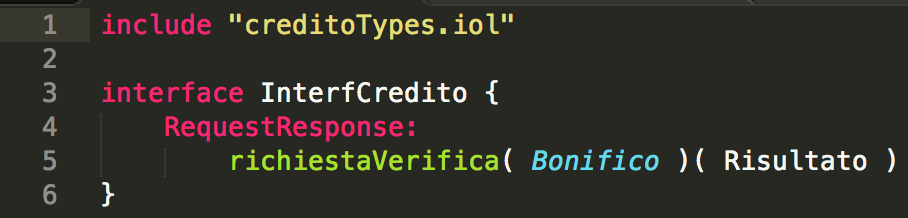
\includegraphics[scale=0.5]{immagini/interfCredito.png}\\
L'unica operazione viene implementata nel file {\tt creditoServer.ol}:
dopo aver ricevuto un bonifico, viene deciso l'esito della verifica
scegliendo un numero casuale (grazie all'interfaccia {\tt Math} di
Jolie). Se il numero scelto \`e minore o uguale di {\tt 0.3}, l'esito
viene settato a {\tt false}, altrimenti a {\tt true}.
Il server contiene poi una {\tt inputPort}, in ascolto sulla porta
{\tt 8200} con protocollo {\tt http}.
Nel file {\tt creditoTypes.iol} vengono descritti i tipi utilizzati.

\subsubsection*{Calcolo Distanze}
Il servizio di calcolo delle distanze viene definito nel file
{\tt interDistanza.iol}, come si pu\`o vedere in figura. \\\\
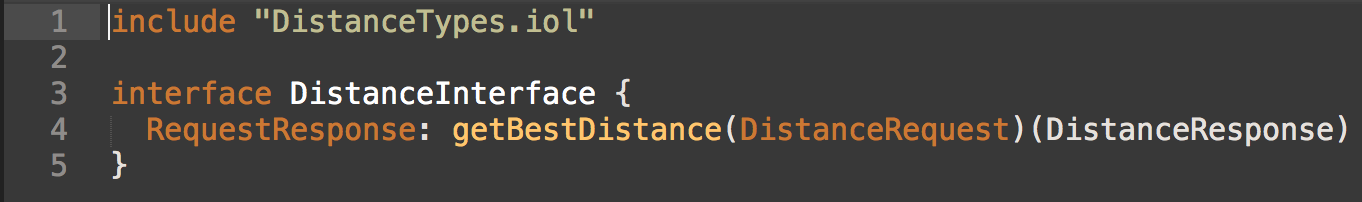
\includegraphics[scale=0.5]{immagini/interfDistanza.png}\\
Il servizio di calcolo delle distanze maschera una chiamata ai servizi
offerti da Google Maps, raggiunti tramite il parametro {\tt location}
impostato a \\
{\tt socket://maps.googleapis.com:80/maps/api/distancematrix/}.
Il servizio prende in input due punti geografici tra i quali calcolare
la distanza, richiedendo per entrambi i parametri contenenti la citt\`a
e la provincia. Una volta che i punti vengono dati al servizio, viene
composta una richiesta per Google Maps, impostando come mezzo di
trasporto la macchina (tramite il parametro {\tt driving}). Il servizio,
ricevuta la risposta, ne estrae le informazioni utili che verranno poi
utilizzate dal sistema.
Nel particolare, il servizio contiene una {\tt outputPort} verso il
servizio di distanze di Google Maps, con protocollo
{\tt http \{.method = ``get''\}}.


\subsubsection*{Ditta di spedizioni}
La ditta di spedizioni ha un'intefaccia semplificata, definita nel file
{\tt interfCorriere.iol}, come si pu\`o vedere in figura. \\\\
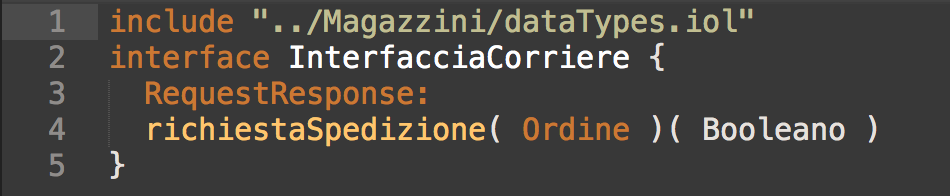
\includegraphics[scale=0.5]{immagini/interfCorriere.png}\\
L'unica operazione viene implementata nel file {\tt corriereServer.ol},
che compone una stringa formattata utilizzando i campi dell'input di
tipo {\tt OrdineSpedizione}.
Il file contiene inoltre una {\tt inputPort}, in ascolto sulla porta
{\tt 8400} con protocollo {\tt http}.
Nel file {\tt corriereTypes.iol} vengono definiti i tipi utilizzati.

\subsubsection*{Fornitore}
Il fornitore ha un'intefaccia semplificata, definita nel file
{\tt interfFornitore.iol}, come si pu\`o vedere in figura. \\\\
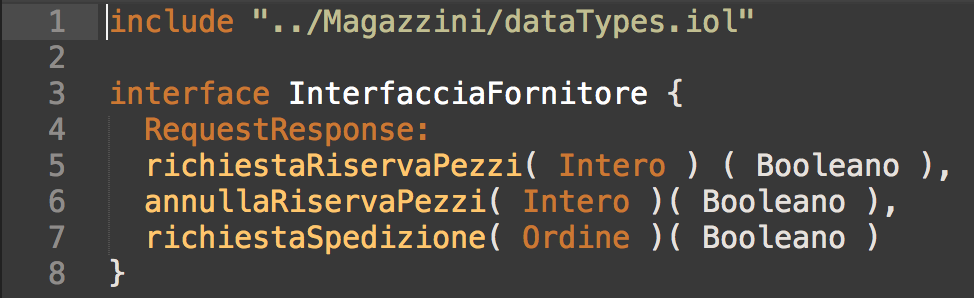
\includegraphics[scale=0.5]{immagini/interfFornitore.png}\\
L'unica operazione viene implementata nel file {\tt fornitoreServer.ol},
che compone una stringa formattata utilizzando i campi dell'input di
tipo {\tt OrdineComponente}.
Il file contiene inoltre una {\tt inputPort}, in ascolto sulla porta
{\tt 8300} con protocollo {\tt http}.
Nel file {\tt fornitoreTypes.iol} vengono definiti i tipi utilizzati.
